% Digital Logic Report Template
% Created: 2020-01-10, John Miller

%==========================================================
%=========== Document Setup  ==============================

% Formatting defined by class file
\documentclass[11pt]{article}

% ---- Document formatting ----
\usepackage[margin=1in]{geometry}	% Narrower margins
\usepackage{booktabs}				% Nice formatting of tables
\usepackage{graphicx}				% Ability to include graphics

%\setlength\parindent{0pt}	% Do not indent first line of paragraphs 
\usepackage[parfill]{parskip}		% Line space b/w paragraphs
%	parfill option prevents last line of pgrph from being fully justified

% Parskip package adds too much space around titles, fix with this
\RequirePackage{titlesec}
\titlespacing\section{0pt}{8pt plus 4pt minus 2pt}{3pt plus 2pt minus 2pt}
\titlespacing\subsection{0pt}{4pt plus 4pt minus 2pt}{-2pt plus 2pt minus 2pt}
\titlespacing\subsubsection{0pt}{2pt plus 4pt minus 2pt}{-6pt plus 2pt minus 2pt}

% ---- Hyperlinks ----
\usepackage[colorlinks=true,urlcolor=blue]{hyperref}	% For URL's. Automatically links internal references.

% ---- Code listings ----
\usepackage{listings} 					% Nice code layout and inclusion
\usepackage[usenames,dvipsnames]{xcolor}	% Colors (needs to be defined before using colors)

% Define custom colors for listings
\definecolor{listinggray}{gray}{0.98}		% Listings background color
\definecolor{rulegray}{gray}{0.7}			% Listings rule/frame color

% Style for Verilog
\lstdefinestyle{Verilog}{
	language=Verilog,					% Verilog
	backgroundcolor=\color{listinggray},	% light gray background
	rulecolor=\color{blue}, 			% blue frame lines
	frame=tb,							% lines above & below
	linewidth=\columnwidth, 			% set line width
	basicstyle=\small\ttfamily,	% basic font style that is used for the code	
	breaklines=true, 					% allow breaking across columns/pages
	tabsize=3,							% set tab size
	commentstyle=\color{gray},	% comments in italic 
	stringstyle=\upshape,				% strings are printed in normal font
	showspaces=false,					% don't underscore spaces
}

% How to use: \Verilog[listing_options]{file}
\newcommand{\Verilog}[2][]{%
	\lstinputlisting[style=Verilog,#1]{#2}
}

\usepackage[section]{placeins}


%======================================================
%=========== Body  ====================================
\begin{document}

\title{ELC 2137 Lab 10: 7-segment Display with Time-Division Multiplexing}
\author{Aaron Mendoza}

\maketitle


\section*{Summary}

Type the summary of your experiment and results here.  





\section*{Results}


\subsection*{Simulation Waveforms}
\begin{figure}[ht]\centering
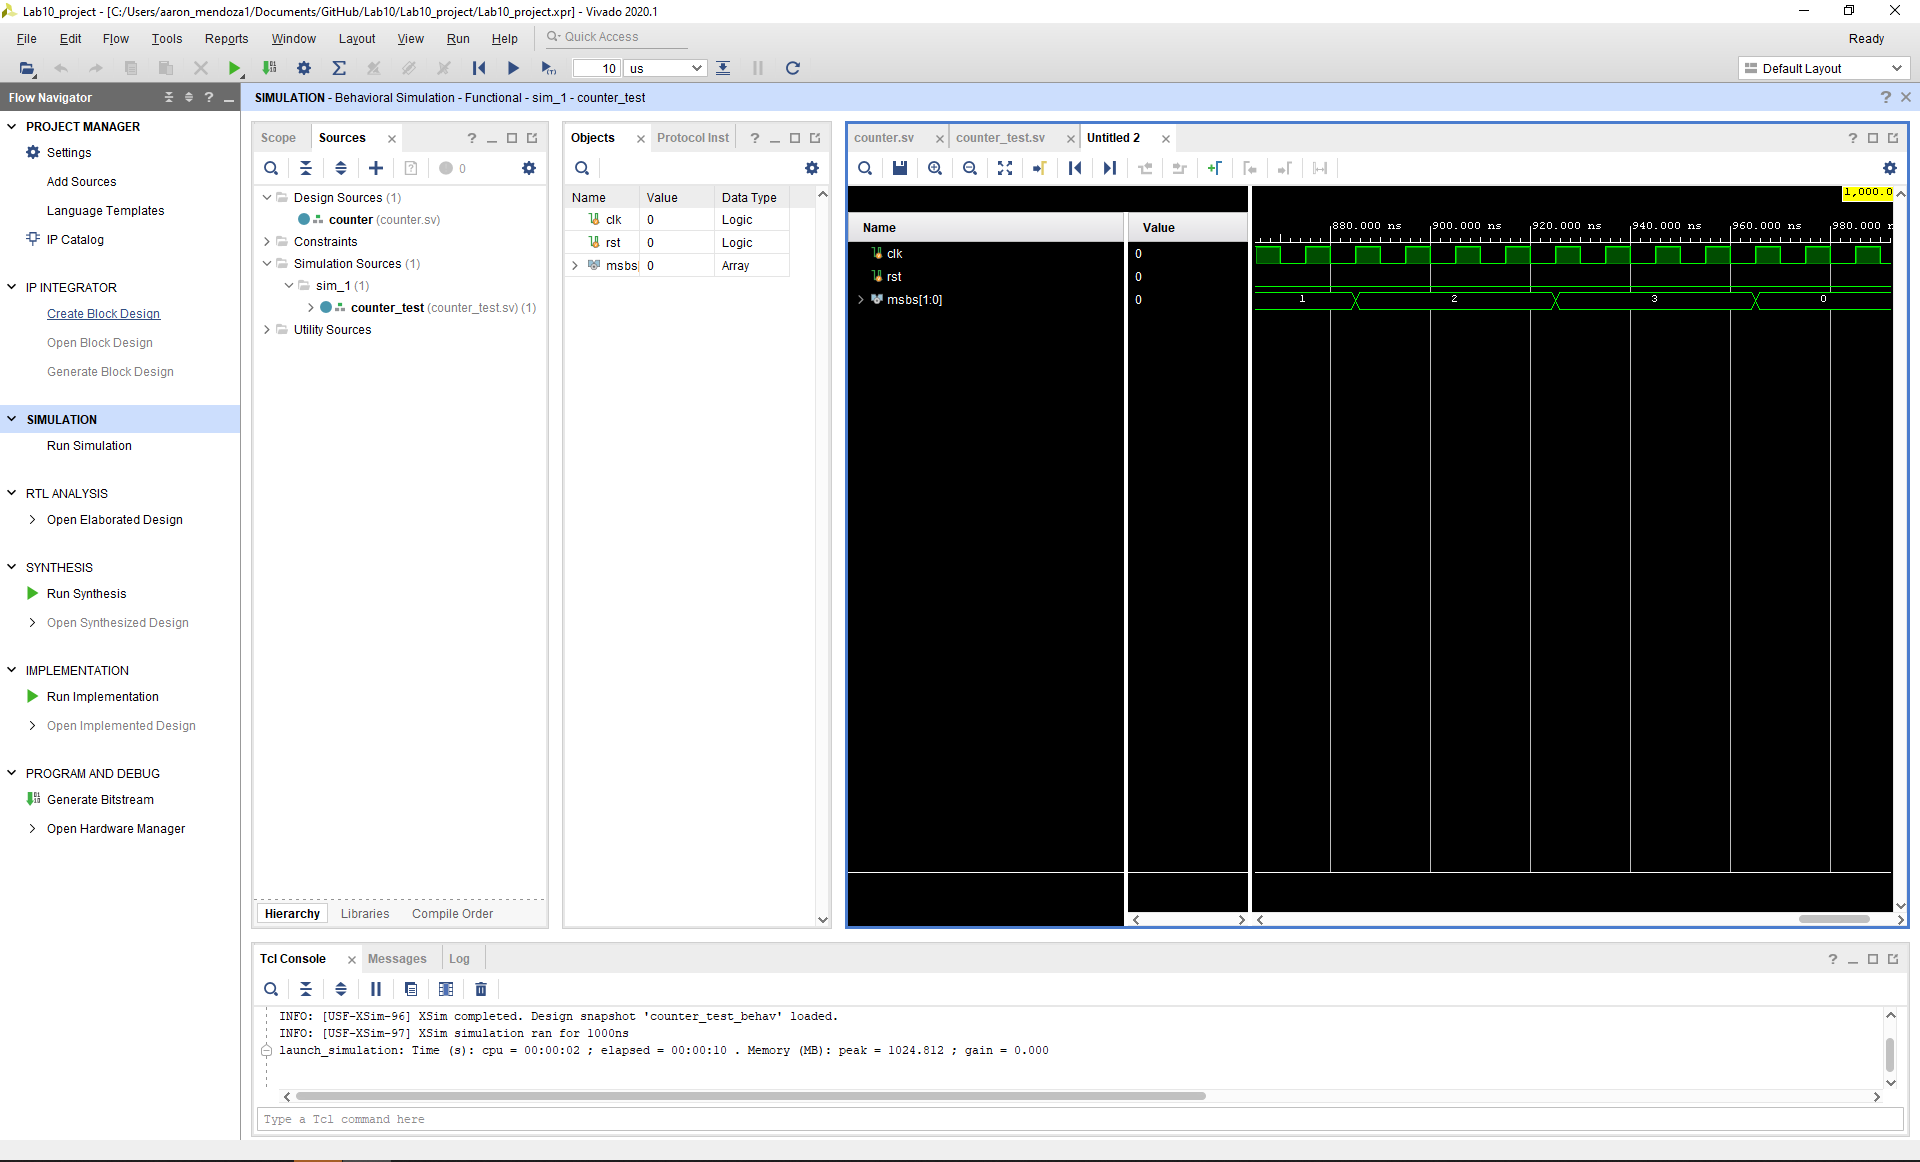
\includegraphics[width=1\textwidth,trim=19cm 15cm 0.5cm 4.5cm,clip]{counter_test_screenshot}
	\caption{Counter Simulation with N=4}
	\label{fig:sim_with_table}
\end{figure}


\begin{figure}[ht]\centering
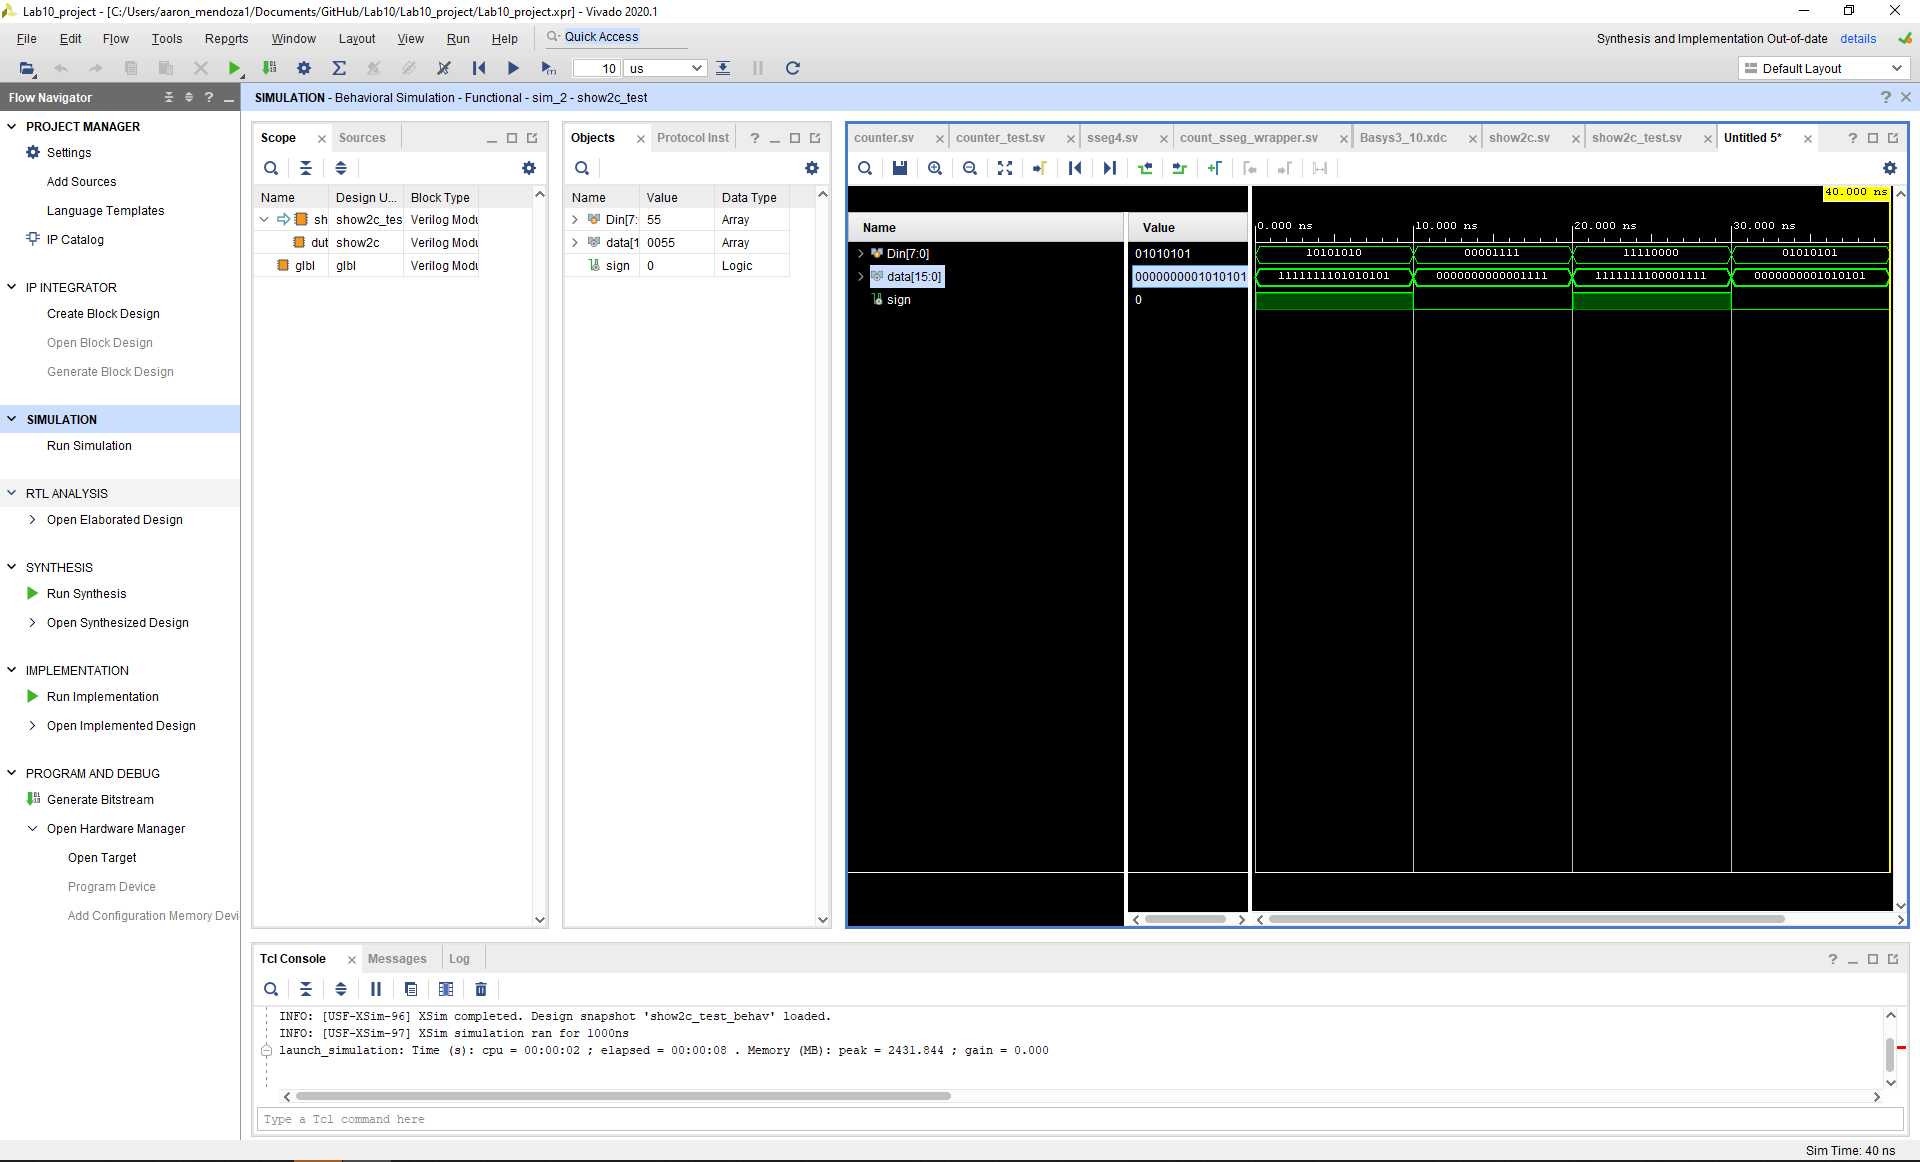
\includegraphics[width=1\textwidth,trim=19cm 15cm 0.5cm 4.5cm,clip]{show2c_test_screenshot}
	\caption{Show 2's Comp Simulation}
	\label{fig:sim_with_table}
\end{figure}

\FloatBarrier

\subsection*{Basys3 Board Pictures}
\begin{figure}[ht]\centering
\includegraphics[width=1\textwidth,trim=15cm 15cm 0.5cm 4.5cm,clip]{count_board}
	\caption{7-seg display after programming the count/sseg wrapper bitstream onto the Basys3 board}
	\label{fig:sim_with_table}
\end{figure}

\begin{figure}[ht]\centering
\includegraphics[width=1\textwidth,trim=15cm 15cm 0.5cm 4.5cm,clip]{pos_number}
	\caption{7-seg display after adding 16 and 9}
	\label{fig:sim_with_table}
\end{figure}


\begin{figure}[ht]\centering
\includegraphics[width=1\textwidth,trim=15cm 15cm 0.5cm 4.5cm,clip]{neg_number}
	\caption{7-seg display after subtracting 32 from 19}
	\label{fig:sim_with_table}
\end{figure}




\section*{Code}

\Verilog[firstline=22, lastline=41, caption=Counter Module Code]{Lab10_project/codedirectory/counter.sv}|

\Verilog[firstline=22, lastline=39, caption=Counter Test Module Code]{Lab10_project/codedirectory/counter_test.sv}|

\Verilog[firstline=22, lastline=48, caption=Counter 7-seg Module Code]{Lab10_project/codedirectory/count_sseg_wrapper.sv}|

\Verilog[firstline=22, lastline=51, caption=Show 2's Comp Module Code]{Lab10_project/codedirectory/show2c.sv}|

\Verilog[firstline=22, lastline=42, caption=Show 2's Comp Test Module Code]{Lab10_project/codedirectory/show2c_test.sv}|

\Verilog[firstline=22, lastline=67, caption=Top-Level Module Code]{Lab10_project/codedirectory/top_level.sv}|


\end{document}
